
\chapter{Publish on server}
\label{chap:publish}

%\nomenclature{SP1}{Service pack 1}
In this appendix is step-by-step tutorial how to publish the project on the Windows Server 2008 R2 Standard x64 SP1.

\section{Creation of publish package}
\label{sec:deployPackage}
This step can be done on developer's work station, not on the server itself.

Creation of the publish package is simple.
Open the solution on the Visual Studio 2010 and in the \emph{Solution explorer} right click on the \emph{Malsys.Web} project and chose \emph{Publish} from the context menu (\autoref{fig:publishVs}).
Then appears popup dialog with publish settings.
In this tutorial we will use publishing to the file system as you can see in \autoref{fig:publishDialog}.
Then click on the \emph{Publish} button and the publish package will be created in selected directory.
Do not forget to set \emph{release} configuration in the Visual Studio 2010 before publishing.

\begin{figure}[h!]
	\subfloat[]{\label{fig:publishVs}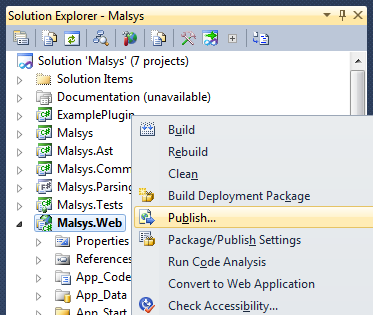
\includegraphics[width=0.5\linewidth]{PublishVs}}
	\hfill
	\subfloat[]{\label{fig:publishDialog}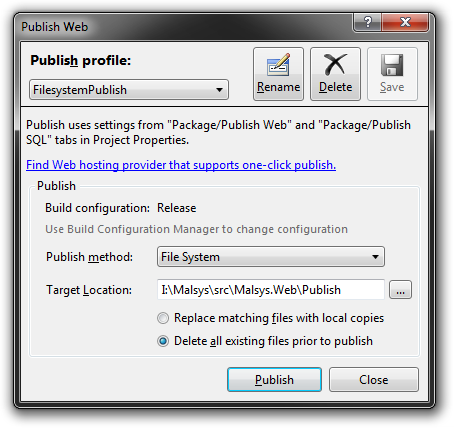
\includegraphics[width=0.46\linewidth]{PublishDialog}}
	\caption{Creation of publish the package in the Visual Studio 2010}
	\label{fig:publish}
\end{figure}
 
 

\section{Configuration of the server}

Following steps expects fresh installation of the Windows Server 2008 R2 Standard x64 SP1.
If any described component is already installed it can be skipped.


\subsection{Internet Information Services (IIS)}

Run the \emph{Server Manager} and in \emph{Roles summary} click on the \emph{Add Roles} button.
Skip the \emph{Before You Begin} page if it appears, select the \emph{Web Server (IIS)} from the list and click the \emph{Next} button.
On \emph{Role Services} screen select \emph{ASP.NET} and \emph{HTTP Redirection} and confirm installation of any dependencies as well.
Then click the \emph{Next} button and finish installation.


\subsection{Web platform installer}

Download the \emph{Web Platform Installer} from \url{http://www.microsoft.com/web/downloads/platform.aspx} and run it.
In the \emph{Web Platform Installer} switch to the \emph{Products} tab and mark to install following products (\autoref{fig:wpi}):
\begin{itemize*}
	\item Microsoft .NET Framework 4
	\item SQL Server Express 2008 R2
	\item ASP.NET MVC 3 (Visual Studio 2010)
	\item ASP.NET WebPages
	\item ASP.NET MVC Tools Update
	\item ASP.NET Web Pages Language Packs Language Packs
	\item URL Rewrite 2.0
	\item IIS: Logging Tools
\end{itemize*}

\begin{figure}[h!]
	\centering
	\subfloat{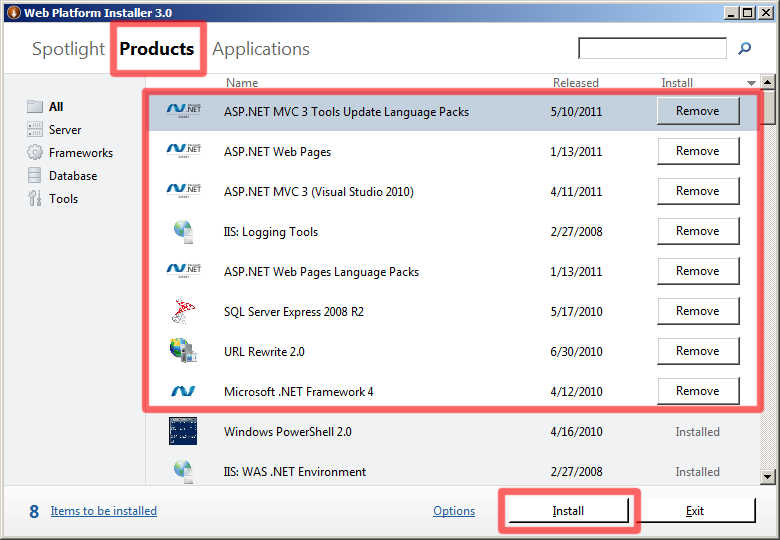
\includegraphics[width=0.8\linewidth]{WebPlatformInstaller}}
	\caption{Marked products to install in the \emph{Web Platform Installer}}
\end{figure}
		
		

\subsection{F\#}

\subsubsection{F\# Redistributable Package}

To load the F\# 4.0 libraries properly the \emph{F\# 2.0 Runtime SP1} must be installed.
The redistributable package can be downloaded from \url{http://msdn.microsoft.com/en-us/library/ee829875.aspx}.

\subsubsection{F\# PowerPack}

Standard F\# distribution do not contain tolls like FsLex and FsYacc which are used in this project.
They are in downloadable package called the \emph{F\# PowerPack} which can be downloaded from \url{http://fsharppowerpack.codeplex.com/}.


\section{Deploy of the application}

In this moment all needed software to run the web is installed on the server.


\subsection{Creation of new App Pool}

Open the \emph{Internet Information Services (IIS) Manager}\footnote{The \emph{Internet Information Services (IIS) Manager} can be easily fond typing "IIS" in the start menu search bar.}, in the left menu open tree node with the name of your server, right click on \emph{Application Pools} and choose \emph{Add Application Pool} from the context menu.
Enter the name (\emph{Malsys} in our case) of new App Pool and as \emph{.NET Framework version} chose \emph{.NET Framework v4.0} (\autoref{fig:newAppPool}).

Then select the \emph{Application Pools} node (left menu), right click on newly created App Pool and chose \emph{Advanced settings}.
In the \emph{Advanced Settings} dialog box find the category called \emph{Process Model}.
The first row in the category will be the \emph{Identity} row.
Click on the \emph{Identity} row and then click on the small button that shows on the right-hand side of the value cell.
A dialog box called \emph{Application Pool Identity} will popup.
Within that dialog box make sure the first radio button titled \emph{Built-in Account} is selected.
In the dropdown box below the radio button choose \emph{Network Service} for the identity.
Then confirm all dialogs with \emph{Ok} buttons.

\begin{figure}[h!]
	\subfloat[New app pool dialog]{
		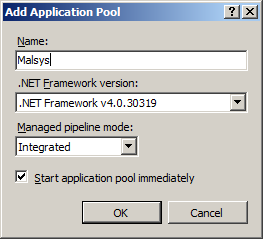
\includegraphics[width=0.4\linewidth]{NewAppPool}
		\label{fig:newAppPool}
	} \hfill
	\subfloat[App pool settings dialog]{
		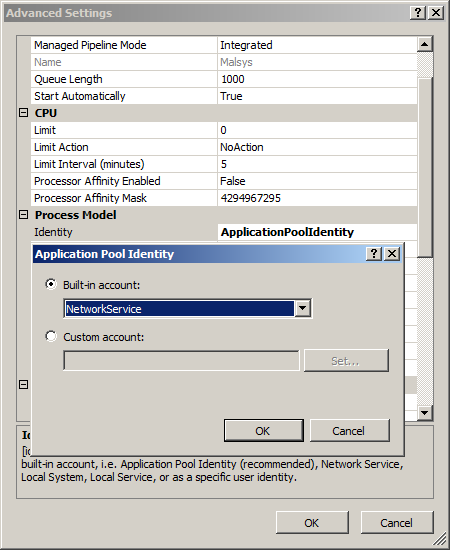
\includegraphics[width=0.5\linewidth]{AppPoolSettings}
		\label{fig:introHTree}
	}
	\caption{App pool settings dialogs}
\end{figure}


\subsection{Creation of new App Pool}

In the \emph{Internet Information Services (IIS) Manager} click on the \emph{Sites} node on the left menu.
If your installation of the IIS is fresh you can delete default site called \emph{Default Site}.
Then right click \emph{Sites} node and chose \emph{Add Web Site}.

In the dialog enter the \emph{Site name} and chose newly created App Pool from previous step.
Then enter physical path of the web root (\emph{C:\textbackslash{}inetpub\textbackslash{}WwwMalsys} in our case).
Then you can configure \emph{Binding}.
If the server will host only this web site we can leave default settings (\autoref{fig:addWebSite}).

\begin{figure}[h!]
	\centering
	\subfloat{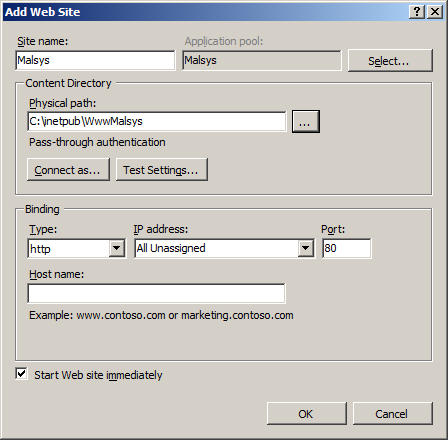
\includegraphics[width=0.6\linewidth]{WebSite}}
	\caption{Filled \emph{Add Web Site} dialog}	
	\label{fig:addWebSite}
\end{figure}


\subsection{Copy files}

\begin{wrapfigure}{r}{0.5\textwidth}%
	\vspace{-1cm}
	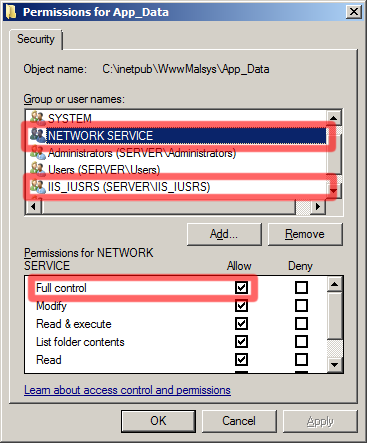
\includegraphics[width=\linewidth]{AppDataRights}
	\caption{Rights of the \emph{App\_Data} directory}
	\label{fig:appDataRights}
\end{wrapfigure}

Copy all files from compiled deployment package created (in \autoref{sec:deployPackage}) to the web site root.
Database file is not included in deployment package to avoid rewriting "life" while updating the web site.
Empty database file is located in the \emph{App\_Data.empty.zip} archive in the \emph{App\_Data} directory of the \emph{Malsys.Web} project.
Extract both files from the archive to the \emph{App\_Data} directory n the web root.

To allow access of database server to the database files set access the \emph{App\_Data} to full control  for users \emph{NETWORK SERVICE} and \emph{IIS\_IUSR} as you can see in \autoref{fig:appDataRights}.

%ensure IIS_IUSR has full control over WorkDir, GalleryWorkDir, ErrorLogs
	
set 























